\documentclass[11pt]{article}
\usepackage[margin=1in]{geometry} 
\usepackage{amsmath}
\usepackage{tcolorbox}
\usepackage{amssymb}
\usepackage{amsthm}
\usepackage{commath}
\usepackage{lastpage}
\usepackage{fancyhdr}
\usepackage{accents}
\usepackage{csquotes}
\usepackage{soul}
\newcommand{\ubar}[1]{\underaccent{\bar}{#1}}
\pagestyle{fancy}
\setlength{\headheight}{40pt}


\newenvironment{solution}
  {\renewcommand\qedsymbol{$\blacksquare$}
  \begin{proof}[Solution]}
  {\end{proof}}
\renewcommand\qedsymbol{$\blacksquare$} 
\begin{document}

\lhead{Yida Liu} 
\rhead{EECS 416 Spring 2020 \\ Convex Optimization for Engineering \\ Homework 7} 
\cfoot{\thepage\ of \pageref{LastPage}}

\newcommand{\mbf}{\mathbf}
\newcommand{\T}{^\intercal}
\newcommand{\partialgx}{\frac{\partial g(\mathbf{x})}{\partial\mathbf{x}}}
\newcommand{\partialgl}{\frac{\partial g(\mathbf{x})}{\partial\mathbf{\lambda}}}


\section{Global Minimizer of Non-convex Problem}

The problem is not convex because the equality constraint is not affine, as we already showed that non-affine equality constraint set are not convex.

Taking the Lagrange multiplier method, and solve for the stationary point with Lagrange multiplier
\[
\left(\begin{array}{c}
{x_1 }^2 +{x_2 }^2 +{x_3 }^2 -1 = 0\\
2\,\lambda \,x_1 -6\,x_1 +2 = 0\\
2\,x_2 +2\,\lambda \,x_2 +2 = 0\\
4\,x_3 +2\,\lambda \,x_3 +2 = 0
\end{array}\right)
\]

Construct the second order test
\[
\nabla^2_{xx}L(x^*, \lambda^*) = \nabla^2f(x^*) + \lambda^* \nabla^2h(x^*) = \left(\begin{array}{ccc}
2\,\lambda -6 & 0 & 0\\
0 & 2\,\lambda +2 & 0\\
0 & 0 & 2\,\lambda +4
\end{array}\right) 
\]
with regard to domain $T(x^*) = \{d | \nabla h(x)^\intercal d = 0\} = \{d | 2x_1d_1 + 2x_2d_2 + 2x_3d_3 = 0\}$. With the domain, we have the $d \in T(x^*)$ as a function of $x^*$, shown as
\[
d(x^*) = \left(\begin{array}{c}
     d_1 \\
     d_2 \\
     \frac{-x_1d_1 - x_2d_2}{x_3}
\end{array}\right)
\]

The from the equation set, we could first express $x$ in $\lambda$ and then solve for $x^*$ from $\lambda^*$, we discuss them accordingly
\begin{enumerate}
% first case
\item $\lambda^* = 0.2235 , \mbf{x^*} = \left(\begin{array}{ccc}
0.3602 & -0.8173 & -0.4497
\end{array}\right)$

\[
d(x^*) = \left(\begin{array}{c}
d_1 \\
d_2 \\
0.8008\,d_1 -1.8173\,d_2 
\end{array}\right)
\]
\[
\nabla^2_{xx}L(x^*, \lambda^*) = \left(\begin{array}{ccc}
-5.5530 & 0 & 0\\
0 & 2.4470 & 0\\
0 & 0 & 4.4470
\end{array}\right)
\]
\[
d^\intercal \nabla^2_{xx}L(x^*, \lambda^*) d = -2.7010\,{d_1 }^2 -12.9441\,d_1 \,d_2 +17.1340\,{d_2 }^2
\]

Not a strict local minimizer.

% second case 
\item $\lambda^* = 1.8919 , \mbf{x^*} =\left(\begin{array}{ccc}
0.1626 & 0.4653 & 0.8701
\end{array}\right)$


\[
d(x^*) = \left(\begin{array}{c}
d_1 \\
d_2 \\
-0.1869\,d_1 -0.5347\,d_2 
\end{array}\right)
\]
\[
\nabla^2_{xx}L(x^*, \lambda^*) = \left(\begin{array}{ccc}
-2.2162 & 0 & 0\\
0 & 5.7838 & 0\\
0 & 0 & 7.7838
\end{array}\right)
\]
\begin{align*}
d^\intercal \nabla^2_{xx}L(x^*, \lambda^*) d &= 93.8025\,{d_1 }^2 -73.5838\,d_1 \,d_2 +19.8815\,{d_2 }^2\\
&= (9.6852d_1 - 3.7988d_2)^2 + 5.4507d_2^2
\end{align*}

\textbf{A strict local minimizer.}

% third case
\item $\lambda^* = -3.1493 , \mbf{x^*} =\left(\begin{array}{ccc}
0.1626 & 0.4653 & 1.3052
\end{array}\right)$

\[
d(x^*) = \left(\begin{array}{c}
d_1 \\
d_2 \\
-0.1246\,d_1 -0.3565\,d_2 
\end{array}\right)
\]
\[
\nabla^2_{xx}L(x^*, \lambda^*) = \left(\begin{array}{ccc}
-12.2986 & 0 & 0\\
0 & -4.2986 & 0\\
0 & 0 & -2.2986
\end{array}\right)
\]
\[
d^\intercal \nabla^2_{xx}L(x^*, \lambda^*) d = -12.3789\,{d_1 }^2 -0.4594\,d_1 \,d_2 -4.9558\,{d_2 }^2
\]

Not a strict local minimizer.


% fourth case
\item $\lambda^* = 4.0352 , \mbf{x^*} =\left(\begin{array}{ccc}
-0.9660 & -0.1986 & -0.1657
\end{array}\right)$

\[
d(x^*) = \left(\begin{array}{c}
d_1 \\
d_2 \\
-5.8299\,d_1 -1.1986\,d_2 
\end{array}\right)
\]
\[
\nabla^2_{xx}L(x^*, \lambda^*) = \left(\begin{array}{ccc}
2.0705 & 0 & 0\\
0 & 10.0705 & 0\\
0 & 0 & 12.0705
\end{array}\right)
\]
\[
d^\intercal \nabla^2_{xx}L(x^*, \lambda^*) d = 412.3126\,{d_1 }^2 +168.6889\,d_1 \,d_2 +27.4114\,{d_2 }^2
\]
\textbf{A strict local minimizer.}

\end{enumerate}

$f(\bm x_4^*) = -5.3655 < f(\bm x_2^*) = -1.5922$. Thus $\bm x_4^*$ is the global minimizer. 

The constraint set is a bounded space. In fact, the space is bounded by a sphere in $\mathbb{R}^3$ of radius 1. By Weierstrass theorem, there must exist a global minimizer for continuous function $f(x)$. In this case, the strict local minimizer shown above would be the global global minimizer for this problem (even though the problem is not convex).

\section{KKT Condition and KKT Point}

We form the Lagrangian using KKT Multipliers
\[
L(\bm{x, \lambda, \mu}) = (x_1 - 1.5)^2 + (x_2 - 0.5)^2 + \mu_1 (x_1 + x_2 - 2) + \mu_2 (x_1^2 + (x_2 - 1)^2 - 1) - \mu_3 x_1
\]

\subsection{KKT Point and Global Minimizer}

This is essentially the proof for the KKT theorem
\[
\text{$x^*$ is a global minimizer} \iff \text{$x^*$ is a KKT point}
\]

\begin{enumerate}
\item Why a KKT point is a global minimizer? (Sufficient condition)
\par First, with a given optimal solution $x^*, \lambda^*, \mu^*$ that satisifies KKT condition, we know that $L(x^*, \lambda^*, \mu^*) = f(x^*)$ due to complementary slackness andfeasibility. In addition, $L(x, \lambda, \mu)$ is convex on the constraint set. We can easily show that, with regard to the gradient at $x^*$ (which is zero), we cannot find a point $x$ such that $L(x, \lambda^*, \mu^*) < L(x^*, \lambda^*, \mu^*)$ within the bounded region. Apart from that, the Weierstrass theorem applies as well, which shows that $x^*$ is the global minimizer. 

\item Why a global minimizer needs to be a KKT point? (Necessary condition)



\end{enumerate}

\subsection{KKT Condition of the Optimization Problem}

\begin{itemize}
\item Gradient
\[
\begin{array}{l}
\mu_1 -\mu_3 +2\,x_1 +2\,\mu_2 \,x_1 -3=0\\
\mu_1 +2\,x_2 +\mu_2 \,{\left(2\,x_2 -2\right)}-1=0\\
\end{array}
\]
\item Feasibility
\[
\begin{array}{l}
     x_1 + x_2 - 2 \leq 0 \\
     x_1^2 + (x_2 - 1)^2 - 1 \leq 0 \\
     - x_1 \leq 0
\end{array}
\]

\item Complementary Slackness
\[
\begin{array}{l}
     \mu_1(x_1 + x_2 - 2) = 0 \\
     \mu_2(x_1^2 + (x_2 - 1)^2 - 1) = 0 \\
     - \mu_3x_1 = 0
\end{array}
\]
\item Non-Negativity
\[
\mu_1, \mu_2, \mu_3 \geq 0
\]
\end{itemize}

We discuss in different cases:
\begin{enumerate}
\item No active constraints.
\par Then $\mu_1, \mu_2, \mu_3 = 0$, gives $(x_1, x_2) = (\frac{3}{2}, \frac{1}{2})$. Violates Feasibility (2).


\item One active constraint: $g_1 = 0$
\par Then $\mu_2, \mu_3 = 0$. Solve the system gives $(x_1, x_2, \mu_1) = (\frac{3}{2}, \frac{1}{2}, 0)$. Violates Feasibility (2).

\item One active constraint: $g_2 = 0$ 
\par Then $\mu_1 = 0, \mu_3 = 0$. Solve for the system, 
\begin{enumerate}
\item $\mu_2 = \frac{\sqrt{10}}{2} - 1$
\par $x_1 = \frac{3}{\sqrt{10}}, x_2 = 1 - \frac{1}{\sqrt{10}}$.\textbf{ A KKT point.}
\item  $\mu_2 = - \frac{\sqrt{10}}{2} - 1$. Violates Non-Negativity.
\end{enumerate}


\item One active constraint: $g_3 = 0$ 
\par Then $\mu_1, \mu_2 = 0, x_1 = 0$. Solve the system gives $(x_1, x_2, \mu_3) = (0, \frac{1}{2}, -3)$. Violate Non-negativity. 

\item Two active constraint: $g_1, g_2 = 0$ 
\par Then $\mu_3 = 0$. Solve for the system
\begin{enumerate}
\item $x_2 = 2$
\par $x_1 = 0, \mu_1 = 3, \mu_2 = -2$. Violates Non-negativity.
\item $x_2 = 1$
\par $x_1 = 1, \mu_1 = -1$. Violates Non-negativity.
\end{enumerate}


\item Two active constraint: $g_2, g_3 = 0$ 
\par Then $\mu_1 = 0$.
We immediately have $x_1 = 0$, $\mu_3 = -3$. Violates Non-Negativity

\item Two active constraint: $g_1, g_3 = 0$ 
\par Then $\mu_2 = 0$. Solve for the system, $(x_1, x_2, \mu_1) = (0, 2, -3)$. Violates Non-Negativity. 

\item All active constraint: $g_i = 0$ 
We immediately have $x_1 = 0$, then $x_2 = 2$. We have $\mu_1 + 2\mu_2 = -3$. Violates Non-Negativity. 

\end{enumerate}

We have only 1 KKT point. Thus the solution $x_1 = \frac{3}{\sqrt{10}}, x_2 = 1 - \frac{1}{\sqrt{10}}$. is the global minimizer. 


\section{Use KKT Theorem on Convex Problem}

The objective funtion is convex: $d^\intercal H d = 2d_1^2 + 2d_2^2 \geq 0 \forall \mathbf{d} \neq 0$ The constraint set is known to be convex as it is bounded by a circle. Thus the problem is convex.

Construct the Lagrangian:
\[
L(\bm{x, \lambda, \mu}) = (x_1 - a)^2 + (x_2 - b)^2 + \mu_1 (x_1^2 + x_2^2 - 1)
\]
We start by listing the KKT Conditions:
\begin{align*}
\text{Gradient:}&\\
& (\mu_1 + 1)x_1 = a \\
& (\mu_1 + 1)x_2 = b \\
\text{Feasibility:}&\\
&x_1^2 +x_2^2 - 1 \leq 0 \\
\text{Complementary Slackness:}&\\
&\mu_1 (x_1^2 + x_2^2 - 1) = 0 \\
\text{Non-Negativity:}&\\
&\mu_1 \geq 0
\end{align*}
Two cases:
\begin{enumerate}
\item No active constraints.
\par Then $u_1 = 0$, meaning that $x^* = (x_1, x_2)^\intercal = (a, b)^\intercal$. In addition, since this is parameterized, we discuss under feasible circumstances:
\begin{align*}
    a^2 + b^2 \leq 1 & \,(\text{Feasibility})\\
    a^2 + b^2 \geq 1 & \,(\text{Parameters})
\end{align*}
In this case, ${x^*}^\intercal x^* = 1$.

\item One active constraint $x_1 + x_2 - 1 = 0$. 
\par Partially solve the system, we have $x_1 = \alpha a, x_2 = \alpha b, \alpha = \frac{1}{\mu_1 + 1}$. Eventually, we can solve $\mu_1 = \pm \sqrt{a^2 + b^2} - 1$. However, $\mu_1 \geq 0$, so we have $\mu_1 = \sqrt{a^2 + b^2} - 1$. Since $a^2 + b^2 \geq 1$, $\mu_1$ here is always greater than zero. Thus, $\alpha = \frac{1}{\sqrt{a^2 + b^2}}$. Since the constraint holds, we always have ${x^*}^\intercal x^* = 1$.
\end{enumerate}

\section{Regular Point, KKT Point and Minimizer}
Lagrangian:
\[
L(\bm{x, \lambda, \mu}) = (x_1 - 1)^2 + x_2^2 + \mu_1 (x_1 + x_2 - 2) + \mu_2(x_1^2 + (x_2 - 1)^2 - 1)
\]
KKT Conditions:
\begin{align*}
\text{Gradient:}&\\
& 2(x_1 - 1) + \mu_1 + 2\mu_2x_1\geq 0\\
& x_1(2(x_1 - 1) + \mu_1 + 2\mu_2x_1) = 0 \\
& 2x_2 + \mu_1 + 2\mu_2(x_2 - 1) = 0\\
\text{Feasibility:}&\\
& x_1 + x_2 - 2 \leq 0\\
& x_1^2 + (x_2 - 1)^2 - 1 \leq 0\\
& -x_1 \leq 0\\
\text{Complementary Slackness:}&\\
& \mu_1(x_1 + x_2 - 2) = 0\\
& \mu_2(x_1^2 + (x_2 - 1)^2 - 1) = 0\\
\text{Non-Negativity:}&\\
& \mu_1,\mu_2 \geq 0
\end{align*}


Second-order test:
\[
\nabla^2_{xx}L(x^*, \lambda^*, \mu^*) = \nabla^2f(x^*) + \lambda^* \nabla^2h(x^*) + \mu^* \nabla^2 g(x*) = \left(\begin{array}{cc}
2\,\mu_2 +2 & 0\\
0 & 2\,\mu_2 +2
\end{array}\right)
\]

\begin{figure}[h]
    \centering
    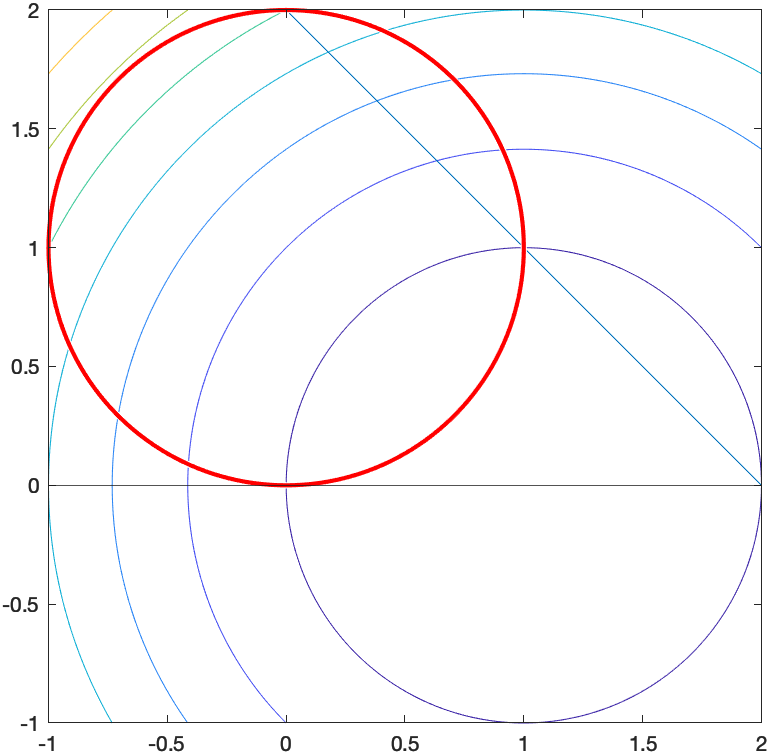
\includegraphics[width=0.5\linewidth]{hw7/prob4_plot.png}
    \label{fig:hw7_prob4_plot}
\end{figure}

\textit{Regular point shown by graphical reasoning.}

\begin{enumerate}
\item (0.5, 1.5)
\par $g_1$ is active. We have $\mu_2= 0$. However, the resulting system is inconsistent if we solve for $\mu_1$. Thus, it is not a KKT point. Therefore not a minimizer.


\item (1, 1)
\par $g_1, g_2$ are active. Solve the system gives $(\mu_1, \mu_2) = (-2, 1)$. Violates Non-negativity. Not a KKT point. Therefore not a minimizer.

\item (0, 2)
\par $g_1, g_2$ are active. We have the system 
\begin{align*}
\mu_1 &\geq 2 \\
\mu_1 + 2\mu_2 &= -4
\end{align*}
Violates Non-Negativity. Not a KKT point. Therefore not a minimizer. 

\end{enumerate}
\section{A Special Form of KKT Conditions}

\subsection{A Special of KKT Condition}
Lagrangian (without non-negativity constraints):
\[
L(\bm{x, \lambda, \mu}) = f(\bm x) + \bm{\lambda}^\intercal (\bm{Ax - b})
\]
We follow the approach stated in page 6, Note 6-2 to formulate this special type of KKT condition. Suppose we have a special multiplier $\gamma$ for the non-negativity constraints. 
\par Lagrangian (with non-negativity constraints):
\[
L(\bm{x, \lambda, \gamma}) = f(\bm x) + \bm{\lambda}^\intercal (\bm{Ax - b}) - \bm\gamma^ \intercal \bm x
\]
Take the gradient with regard to $\bm x$,
\[
\nabla f(\bm x) + \bm A ^\intercal \lambda - \bm\gamma = 0
\]
Or
\[
\bm \gamma  = \nabla f(\bm x) + \bm A ^\intercal \bm\lambda
\]
In addition, with the new multiplier, we have Non-negativity $\bm \gamma \geq 0$ and complementary slackness $\bm \gamma^\intercal \bm x = 0$. By substitution, we formulate this special KTT condition as follows
\begin{align*}
\text{Gradient:}&\\
&\nabla f(\bm x) + \bm A ^\intercal \bm \lambda > 0\\
&\bm x (\nabla f(\bm x) + \bm A ^\intercal \bm \lambda)  =  0 \\
& (\text{No need to do $\forall k \not\in K$ here since all $x \geq 0$.})\\
\text{Feasibility:}&\\
&\bm{Ax - b} = 0\\
& -\bm x \leq 0\\
\end{align*}

Sufficiency: Since $f(x)$ is convex, and the region is bounded, the proof shown for regular convex optimization problem with KKT sufficiency still applies such that we cannot find any $x$ that has a smaller objective value comparing to that of $x^*$.

Necessity: The necessary condition still holds since the Linearity CQ holds for this type of problem. That is to say, the affine prob


\subsection{A Real Problem}

It is easy to show that the problem is convex: all $x_i$ are to the power of 2, which is known to be convex functions and the positive composition of convex functions are still convex. In addtion, the constarints are affine. Thus, we can use the property shown in (5.1) to solve this.
\par Lagrangian:
\[
L = 0.5(x_1 - 2)^2 + 2(x_2 + 4)^2 + (x_3 - 1)^2 + \lambda_1(3x_1 - x_2 -2x_3 - 1) + \lambda_2 (-x_1 + x_2 +x_3 - 2)
\]
\par KKT Condition:
\begin{align*}
\text{Gradient:}&\\
&(x_1 -2) +  3\lambda_1  - \lambda_2 \geq 0 \\
& 4 (x_2 + 4) - \lambda_1 + \lambda_2 \geq 0 \\
& 2(x_3 - 1) -2\lambda_1 + \lambda_2 \geq 0 \\
& ((x_1 -2) +  3\lambda_1  - \lambda_2) x_1 = 0 \\
& (4 (x_2 + 4) - \lambda_1 + \lambda_2)x_2 = 0 \\
& (2(x_3 - 1) -2\lambda_1 + \lambda_2) x_3 = 0 \\
\text{Feasibility:}&\\
& 3x_1 - x_2 -2x_3 - 1 = 0\\
& -x_1 + x_2 +x_3 - 2 = 0 \\
& -x_1, -x_2, -x_3 \leq 0\\
\end{align*}
\par Second-order Test:
\[
\nabla^2_{xx}L(x^*, \lambda^*) = \left(\begin{array}{cc}
1 & 0\\
0 & 4
\end{array}\right)
\]

We discuss the problem into cases when constraints are active or not.
\begin{enumerate}
\item No bound active.
\par Meaning that all $x \neq 0$, and therefore the first part of Gradient (4), (5), (6) equals zero. We have a system of 5 equations and 5 unknowns. Solve the system gives $(x_1, x_2, x_3, \lambda_1, \lambda_2) = (4.1538, 0.8462, 5.3077, -10.7692, -30.1538)$. \textbf{A KKT point}.

\item $g_1$ active.
\par We have $x_1 = 0$. Solve for the system, we have $(x_2, x_3, \lambda_1, \lambda_2) = (5, -3, -14.6667, -21.3333)$. However, $x_3 \leq 0$. Does not satisfy the Non-negativity.

\item $g_2$ active.
\par We have $x_2 = 0$. Solve for the system, we have $(x_1, x_3, \lambda_1, \lambda_2) = (5, 7, -15, -42)$. Violates Gradient (2).

\item $g_3$ active
\par We have $x_3 = 0$. Solve for the system, we have $(x_1, x_2, \lambda_1, \lambda_2) = (1, 3, -6.75, -21.25)$. Violates Gradient (3).

\end{enumerate}

For the lone KKT point $x^* = (4.1538, 0.8462, 5.3077)$, 2nd-order test is pd. Thus, it is a strict local minimizer. This problem is convex, so it is also the global minimizer. 


\section{When KKT Conditions is Useless}
\begin{figure}[h]
    \centering
    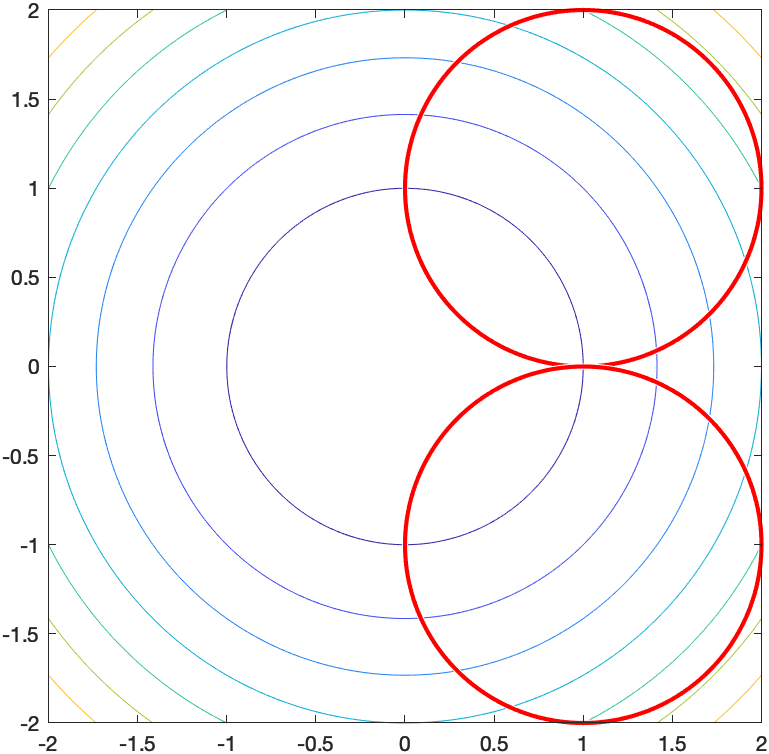
\includegraphics[width=0.5\linewidth]{hw7/prob6_plot.png}
    \label{fig:hw7_prob6_circle}
\end{figure}
As shown in Figure \ref{fig:hw7_prob6_circle}, the feasible region is the intersection of the two unit circle at $(1, 1)$ and $(1, -1)$, which contain only 1 point $(1, 0)$. In this sense, $x^*=(1, 0)$ and $f(x^*) = 1$.
\par Lagrangian:
\[
L(x, \mu) = x_1^2 + x_2^2 + \mu_1((x_1 -1)^2 + (x_2 - 1)^2 - 1) + \mu_2((x_1 -1)^2 + (x_2 + 1)^2 - 1)
\]
\par KKT Condition:
\begin{align*}
\text{Gradient:}&\\
&2x_1 + 2\mu_1(x_1 - 1) + 2\mu_2 (x_1 - 1) = 0 \\
&2x_2 + 2\mu_1(x_2 - 1) + 2\mu_2(x_2 + 1) = 0 \\
\text{Feasibility:}&\\
&(x_1 -1)^2 + (x_2 - 1)^2 - 1 \leq 0\\
&(x_1 -1)^2 + (x_2 + 1)^2 - 1 \leq 0\\
\text{Complementary Slackness:}&\\
&\mu_1((x_1 -1)^2 + (x_2 - 1)^2 - 1) = 0\\
&\mu_2((x_1 -1)^2 + (x_2 + 1)^2 - 1) = 0 \\
\text{Non-Negativity:}&\\
&\mu_1, \mu_2 \geq 0
\end{align*}

Check $x^* = (1, 0)$, we have $g_1, g_2 = 0$. Plugging in the values gives an inconsistent system suggesting $2 = 0$. 
\par \textit{The gradient of $g_1$ and $g_2$ on the optimal point is shown on the plot.}
\par The feasible ``region'' consist of just one point, which means that this lone optima is not a regular point. 

\end{document}

